\section{Modelling}

- detail the structure of the model, eg. the training was called in a notebook (main.ipynb) but the training and the model was defined in discrete python files of their own in accordance with modularity best practices.

\subsection{Model Structure and Hyperparameter Tuning}

The model is a convolutional neural network (CNN) designed for binary image classification. It accepts full-size images of shape $(512, 512, 3)$, which are downscaled to $(256, 256, 3)$ for computational efficiency. The architecture consists of two convolutional layers, each followed by a pooling layer (either max or average pooling, chosen as a hyperparameter) and optional dropout for regularization. After flattening, a dense layer with tunable units and optional dropout is added, followed by a single sigmoid output neuron for binary classification.

Key hyperparameters include the number of filters and kernel sizes in each convolutional layer, pooling type, dropout usage and rates, dense layer units, optimizer type, and learning rate. The model uses either Adam or RMSprop optimizers, with the learning rate also being tunable.

Early stopping is employed to prevent overfitting by monitoring validation loss and restoring the best weights if no improvement is seen for 5 epochs.

\subsection{Hyperparameter Tuning with Hyperband}

The Keras Tuner's Hyperband algorithm is used for hyperparameter optimization. Hyperband efficiently allocates resources by quickly eliminating poorly performing configurations and focusing on promising ones, thus saving computational time compared to exhaustive search. Its main strength is the ability to explore a large hyperparameter space efficiently. However, it may miss optimal configurations if the early stopping criteria are too aggressive or if the search space is not well-defined.

\begin{table}[h]
\centering
\caption{Tunable Hyperparameters}
\begin{tabular}{ll}
\toprule
\textbf{Hyperparameter} & \textbf{Range/Choices} \\
\midrule
filters1         & 32 to 128 (step 16) \\
kernel1          & 3, 5 \\
layer\_1\_pool\_type & max, avg \\
dropout1         & 0.1 to 0.5 (if used) \\
filters2         & 32 to 128 (step 16) \\
kernel2          & 3, 5 \\
layer\_2\_pool\_type & max, avg \\
dense\_units     & 64 to 256 (step 32) \\
dropout2         & 0.1 to 0.5 (if used) \\
optimizer        & adam, rmsprop \\
learning rate    & $1\times10^{-5}$ to $1\times10^{-2}$ (log scale) \\
\bottomrule
\end{tabular}
\end{table}


\section{Model Evaluation and Deployment}


\begin{figure}[h]
    \centering
    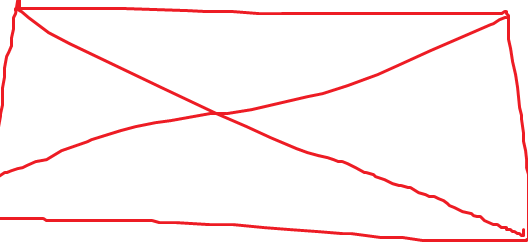
\includegraphics[width=200px]{figures/placeholder.png} % Image filename
    \centering
    \caption{Evidence of an endpoint in Sagemaker} % Caption
    \label{fig:endpoint} % Label
\end{figure}

\begin{figure}[h]
    \centering
    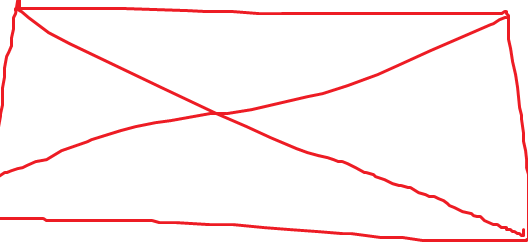
\includegraphics[width=200px]{figures/placeholder.png} % Image filename
    \centering
    \caption{Confusion Matrix} % Caption
    \label{fig:confusion_matrix} % Label
\end{figure}



Using an endpoint, the model was then evaluated on its precision, recall, f1 score, and accuracy. \Cref{fig:endpoint} shows the endpoint configuration in Sagemaker. This allowed for evaluation of the models performance, whilst not being limited by the RAM limitations of the notebook environent in Sagemaker studio. \Cref{fig:confusion_matrix} presents the confusion matrix for the model's predictions. It can be seen that \note{continue here}


\section{Transfer Learning}

The list of the possible CNN structures available for use for transfer learning can be seen in \cite{keras_applications}. Of these, it was reasoned that \note{this model} would be \note{either well suited to the characteristics of the dataset or just an effective model for its computational cost, therefore being a candidate for its ability to demonstrate transfer learning with the intention of finding a higher parameter/computational cost model down the track}